%%%%%%%%%%%%%%%%%%%%%%%%%%%%%%%%%%%%%%%%%
% Short Sectioned Assignment LaTeX Template Version 1.0 (5/5/12)
% This template has been downloaded from: http://www.LaTeXTemplates.com
% Original author:  Frits Wenneker (http://www.howtotex.com)
% License: CC BY-NC-SA 3.0 (http://creativecommons.org/licenses/by-nc-sa/3.0/)
%%%%%%%%%%%%%%%%%%%%%%%%%%%%%%%%%%%%%%%%%

%----------------------------------------------------------------------------------------
%	PACKAGES AND OTHER DOCUMENT CONFIGURATIONS
%----------------------------------------------------------------------------------------

\documentclass[paper=a4, fontsize=11pt]{scrartcl} % A4 paper and 11pt font size

% ---- Entrada y salida de texto -----

\usepackage[T1]{fontenc} % Use 8-bit encoding that has 256 glyphs
\usepackage[utf8]{inputenc}
%\usepackage{fourier} % Use the Adobe Utopia font for the document - comment this line to return to the LaTeX default

% ---- Idioma --------

\usepackage[spanish, es-tabla]{babel} % Selecciona el español para palabras introducidas automáticamente, p.ej. "septiembre" en la fecha y especifica que se use la palabra Tabla en vez de Cuadro

% ---- Otros paquetes ----

\usepackage{url} % ,href} %para incluir URLs e hipervínculos dentro del texto (aunque hay que instalar href)
\usepackage{amsmath,amsfonts,amsthm} % Math packages
%\usepackage{graphics,graphicx, floatrow} %para incluir imágenes y notas en las imágenes
\usepackage{graphics,graphicx, float} %para incluir imágenes y colocarlas

% Para hacer tablas comlejas
%\usepackage{multirow}
%\usepackage{threeparttable}

%\usepackage{sectsty} % Allows customizing section commands
%\allsectionsfont{\centering \normalfont\scshape} % Make all sections centered, the default font and small caps

\usepackage{fancyhdr} % Custom headers and footers
\pagestyle{fancyplain} % Makes all pages in the document conform to the custom headers and footers
\fancyhead{} % No page header - if you want one, create it in the same way as the footers below
\fancyfoot[L]{} % Empty left footer
\fancyfoot[C]{} % Empty center footer
\fancyfoot[R]{} % Page numbering for right footer
\renewcommand{\headrulewidth}{0pt} % Remove header underlines
\renewcommand{\footrulewidth}{0pt} % Remove footer underlines
\setlength{\headheight}{13.6pt} % Customize the height of the header

\numberwithin{equation}{section} % Number equations within sections (i.e. 1.1, 1.2, 2.1, 2.2 instead of 1, 2, 3, 4)
\numberwithin{figure}{section} % Number figures within sections (i.e. 1.1, 1.2, 2.1, 2.2 instead of 1, 2, 3, 4)
\numberwithin{table}{section} % Number tables within sections (i.e. 1.1, 1.2, 2.1, 2.2 instead of 1, 2, 3, 4)

\setlength\parindent{0pt} % Removes all indentation from paragraphs - comment this line for an assignment with lots of text

\newcommand{\horrule}[1]{\rule{\linewidth}{#1}} % Create horizontal rule command with 1 argument of height


\usepackage{hyperref}
\usepackage{listings}
\usepackage{xcolor}
\usepackage{caption}
\usepackage{subcaption}
\usepackage{lmodern}
\usepackage{graphicx}
\usepackage{biblatex}
\usepackage{array}
\usepackage{wrapfig}

\definecolor{codegreen}{rgb}{0,0.6,0}
\definecolor{codegray}{rgb}{0.5,0.5,0.5}
\definecolor{codepurple}{rgb}{0.58,0,0.82}
\definecolor{backcolour}{rgb}{0.95,0.95,0.92}
\usepackage[margin=0.7in]{geometry}

\newcolumntype{C}[1]{>{\centering\arraybackslash}p{#1}}
\newcolumntype{L}[1]{>{\raggedright\arraybackslash}p{#1}}
\newcolumntype{R}[1]{>{\raggedleft\arraybackslash}p{#1}}

\lstdefinestyle{mystyle}{
    backgroundcolor=\color{backcolour},   
    commentstyle=\color{codegreen},
    keywordstyle=\color{magenta},
    numberstyle=\tiny\color{codegray},
    stringstyle=\color{codepurple},
    basicstyle=\ttfamily\footnotesize,
    breakatwhitespace=false,         
    breaklines=true,                 
    captionpos=b,                    
    keepspaces=true,                 
    numbers=left,                    
    numbersep=5pt,                  
    showspaces=false,                
    showstringspaces=false,
    showtabs=false,                  
    tabsize=2
}


\title{	
\normalfont \normalsize 
\textsc{\textbf{Metaheurística grupo 2 (2021-2022)} \\ Grado en Ingeniería Informática \\ Universidad de Granada} \\ [25pt] % Your university, school and/or department name(s)
\horrule{0.5pt} \\[0.4cm] % Thin top horizontal rule
\huge Cuckoo Search \\
Mínima dispersión diferencial \\ % The assignment title
\horrule{2pt} \\[0.5cm] % Thick bottom horizontal rule
}

\author{José María Ramírez González\\\href{mailto:jmramirez@correo.ugr.es}{jmramirez@correo.ugr.es}} % Nombre y apellidos

\date{\normalsize\today} % Incluye la fecha actual

\begin{document}

\maketitle % Muestra el Título

\newpage %inserta un salto de página

\tableofcontents % para generar el índice de contenidos

\newpage

\section{Descripción del problema}

El problema escogido es el conocido como \textit{mínima dispersión diferencial} o \textit{minimum differential dispersion} en inglés.

En este problema se intenta minimizar la dispersión entre un subconjunto $M$ de elementos de un conjunto $C$. Es un problema \textbf{NP-completo}, por lo que resulta inviable resolverlo de manera óptima en un tiempo decente en casos donde $|C|$ o $|M|$ sean grandes.

Nuestro objetivo es encontrar $M \subset C$, y se nos proporcionarán varios casos, cada uno con un $C$ y un $m =|M|$.
En cada caso nos dan, además, la distancia de un elemento al resto de ellos, tal que podamos calcular el \textit{$\Delta$-value} de cada elemento como $\displaystyle \Delta \text{-value}_i = \sum_{j \in M}d_{ij}\quad \forall \, i \in M$, donde $d_{ij}$ es la distancia del elemento $i$ al elemento $j$.

Para calcular la dispersión, realizamos el siguiente cálculo $disp = max(\Delta\text{-value})-min(\Delta\text{-value})$. Esa sería la dispersión asociada a una posible solución $M$, el máximo de sus $\Delta$-values menos el mínimo de ellos. Así pues, nuestra función a minimizar es esa.

Es importante destacar que la dispersión de cada conjunto solución $M$ depende de cada uno de los elementos $w \in M$ y que, cambiando tan solo uno de ellos, esta puede cambiar radicalmente.

\section{Elementos no relativos al algoritmo empleados en la resolución del problema}
Para resolver este problema, hemos implementado el \href{https://en.wikipedia.org/wiki/Cuckoo_search}{\textit{Cuckoo Search}}, un algoritmo con bastante historia, ya que se desarrolló en 2009, y una versión de algoritmo memético que utiliza este algoritmo de búsqueda como componente exploratorio, junto con una búsqueda local para mejorar la explotación.A su vez, vamos a hacer uso de los algoritmos usados en las prácticas 1 a 3 para que nos sirvan de punto de comparación con el \textit{Cuckoo Search}.

Vamos a comentar algunos elementos que no tratan puramente sobre el algoritmo, pero nos ayudarán a comprender pseudocódigo y detalles relativos a la implementación.

\subsection{Representación de los datos}

Los datos de entrada se nos proporcionan en un fichero con la estructura apreciable en el listing \ref{lst:estructuraFicheros}.

\begin{lstlisting}[frame=single,caption={Estructura de los ficheros proporcionados},label=lst:estructuraFicheros, captionpos=b]
n m
0 1 value
0 2 value
...
n-2 n-1 value
\end{lstlisting}

Donde $m = |M|$, $n = |C|$ y \textit{value} es el coste de ir de la posición que aparece primero a la posición que aparece en segundo lugar. En nuestro caso, guardaremos esta información en forma de matriz cuadrada $n \times n$, donde dejaremos 0s en la diagonal principal.

El funcionamiento general de la lectura de los datos sería el representado en el listing \ref{lst:funcionamientoLeerDatos}.

\begin{lstlisting}[frame=single, caption={Generalización de la lectura de los datos},label=lst:funcionamientoLeerDatos, captionpos=b]
archivo = open(archivoConDatos)
n, m = archivo.get(0,1)
matriz = nuevaMatriz(n x n, 0) # Nueva matriz n*n de 0s
for linea in archivo:
    pos1 = linea[0]
    pos2 = linea[1]
    valor = linea[2]
    matriz[pos1][pos2] = valor
    matriz[pos2][pos1] = valor
\end{lstlisting}


\subsection{Representación de la solución}

Para representar los elementos seleccionados, vamos a contar con un vector de tamaño $n$, donde los elementos seleccionados tendrán valor $1$ y los no seleccionados, valor $0$.

Es importante destacar que para que una solución sea válida, el vector solución tiene que tener tantos $1$s como el valor de $m$.

Con este vector y con la matriz de datos podemos calcular la dispersión para una posible solución.


\subsection{Función objetivo}

Nuestro objetivo es minimizar la dispersión de la solución final.
La dispersión se define como la diferencia entre el mayor $\Delta$-value y el menor $\Delta$-value.
El $\Delta$-value está asociado a cada posición seleccionada, de tal forma que $\Delta$-value$_{i} = \sum_{k=0}^{m}datos[i][k]$, es decir, la suma de las distancias de cada elemento seleccionado al resto de elementos seleccionados. Por tanto, nuestra Disp$_i$ sería el mayor de estos valores menos el menor.

A la sumatoria anterior vamos a darle el nombre de \texttt{calcularDvalue}.

Para calcular la dispersión, tan solo tenemos que hacer lo definido en el listing \ref{lst:calcDisp}:

\begin{lstlisting}[frame=single, caption={Cálculo de la dispersión para una posible solución}, captionpos=b, label=lst:calcDisp]
pesosSolucion = []
para seleccion en Solucion: # Donde solucion es un vector
    pesosSolucion += calcularDvalue(seleccion)

ordenar(pesosSolucion)
Dispersion = pesosSolucion.last() - pesosSolucion.first()
\end{lstlisting}



\subsection{Selección de los datos de entrada}

Para seleccionar los datos de entrada, hacemos uso de la librería \textit{os} con la que, introduciendo el nombre de la carpeta donde tenemos todos los archivos con los datos de entrada, nos leerá los nombres de los mismos.

Una vez tengamos los nombres, los ordenamos de menor a mayor con una función que hemos creado y pasamos a ejecutar un bucle que realiza todos los algoritmos para cada archivo.

Podemos encontrar el pseudocódigo en el listing \ref{lst:lecturaArchivos}.

\begin{lstlisting}[frame=single, caption={Versión búsqueda local}, captionpos=b, label=lst:lecturaArchivos]
archivos = leerCarpeta(nombreCarpeta)
ordenarPorNombre(archivos)
para cada archivo en archivos:
    leer(archivo)
    Ejecutar algoritmos
\end{lstlisting}


\subsection{Aleatoriedad en los algoritmos}

Todos los algoritmos implementados en esta práctica utilizan números aleatorios.

Para obtener esta aleatoriedad vamos a hacer uso tanto del paquete \texttt{random} como de \texttt{numpy.random}.

Esto provocará que nuestros algoritmos obtengan resultados distintos en cada ejecución.

\subsection{Medición del tiempo de ejecución}

Para medir los tiempos de ejecución de cada algoritmo, hemos hecho uso de la librería \textit{time}, la cual nos proporciona el tiempo de CPU que tarda en ejecutarse una determinada parte del código con una implementación similar a la del listing \ref{lst:tiempoCPU}.

\begin{lstlisting}[frame=single, caption={Tiempo de ejecución de un programa}, captionpos=b, label=lst:tiempoCPU]
tiempoinicio = tiempoActual()

...
#Ejecucion del algoritmo
...

tiempoFinal = tiempoActual()
tiempoEjecucion = tiempoFinal - tiempoInicio
\end{lstlisting}

\subsection{Generador de soluciones}

Al comenzar la ejecución el algoritmo, vamos a necesitar una o varias soluciones iniciales.

Para generar una posible solución, simplemente vamos a generar un vector de tamaño $n$ sin elementos seleccionados y a seleccionar aleatoriamente $m$ elementos de ese vector.
Esa solución será factible.

Podemos ver una implementación de este generador de soluciones en el listing \ref{lst:generarSol}

\begin{lstlisting}[frame=single, caption={Generador de soluciones}, captionpos=b, label=lst:generarSol]
solucion = [0,0,0,0,0,...,0]  # n 0s

indices = seleccionar m elementos de [0,1,...,n-1] aleatoriamente

solucion[indices] = 1

return solucion
\end{lstlisting}

\subsection{Operador de reparación}

Debido a la forma que hemos implementado nuestros \href{https://en.wikipedia.org/wiki/Lévy_flight}{\textit{Lévy flights}}, nos pueden quedar soluciones que no sean factibles (en nuestro caso, que el número de $1$s sea mayor que $m$), por lo que tendremos que reparalas.

Esto se realiza eliminando de la posible solución aquellos elementos que añadan la mayor dispersión hasta tener exactamente $m$ $1$s.

Podemos ver la implementación en pseudocódigo en el listing \ref{lst:repSol}.

\begin{lstlisting}[frame=single, caption={Reparador de soluciones}, captionpos=b, label=lst:repSol]
if not esSol(sol):
	while numerodeunos(sol) < self.m:
                    media = self.get_media(Solucion)
                    index = self.get_most_impacting_element(Solucion, media)
                    Solucion[index] = 0
\end{lstlisting}

\newpage

\section{\textit{Cuckoo Search}}

Este algoritmo consiste en simular el curioso comportamiento de estos pájaros en la naturaleza, que se dedican a poner huevos en los nidos de otras especies para que cuiden de sus crías. Este parasitismo tiene dos posibles desenlaces: o bien el huésped se da cuenta y abandona el nido/no cuida a la cría o el huésped mantiene a la cría y esta prospera.

En nuestra implementación nos hemos limitado a tener una población estable de huevos de estos pájaros, cada cual representa una solución. Las soluciones peor adaptadas, van a ser descubiertas por los huéspedes, por lo que otros pájaros pondran nuevos huevos en otros nidos.

Una solución aleatoria de cada iteración crecerá y realizará un vuelo Lévy, el cual nos dará un conjunto de pasos con $n$ dimensiones. Usaremos el mayor paso de este conjunto para establecer un umbral de la forma $umbral = max(pasos)*0.1$, tal que los índices cuyo valor de los pasos se encuentren en $(-umbral, umbral)$ se pondrán a $1$.

Esta nueva solución aleatoria, volará hasta otro nido aleatoriamente donde se comparará con la solución que se encuentre allí y, si es mejor, la sustiturá.

Haremos 500 iteraciones de este proceso, debido al alto coste computacional del mismo.

Podemos ver una implementación en pseudocódigo en el listing \ref{lst:cs_simple}.

\begin{lstlisting}[frame=single, caption={Cuckoo search}, captionpos=b, label=lst:cs_simple]
while iters < max_iters and best_nest_disp != 0:
    iters+=1

    Barajar(nests)     
    nest = levy(random(0, n)) # Levy flight

    alet = random(0, n) # Numero aleatorio entre 0 y n

    if calcular_disp(nest) < calcular_disp(nests[alet]):
        nests[alet] = nest # Sustituye
    
    OrdenarPorDisp(nests, Inverso) # Ordena en orden inverso

    disp_mejor_actual = calcular_disp(nests.ultimo)
    if disp_mejor_actual < best_nest_disp:
        best_nest = self.nests.ultimo
        best_nest_disp = disp_mejor_actual

    for i in range(toAbandon):	# Numero de nidos descubiertos
        nests[i] = generar_Sol()
        if calcular_disp(nests[i]) < best_nest_disp:
            best_nest = nests[i]
            best_nest_disp = disp_mejor_actual
            
return best_nest
\end{lstlisting}

Como vemos, el algoritmo no tiene mucha complicación, siendo bastante similar a un genético.

\newpage

\section{Hibridación \textit{Cuckoo Search} y memético}

Vamos a hibridar el algoritmo expuesto en el apartado anterior para que actúe de componente exploratoria en nuestro algoritmo memético desarrollado en la práctica 3.

Consistirá en realizar todo lo expuesto en el apartado anterior, pero añadiéndole un paso de explotación en forma de búsqueda local.

Usaremos el algoritmo memético tal que solo se le aplique la búsqueda local a los $10\%$ mejores nidos.

Podemos ver una implementación en el listing \ref{lst:cs_mem}.

\begin{lstlisting}[frame=single, caption={Hibridación Cuckoo Search y memético}, captionpos=b, label=lst:cs_mem]
while iters < max_iters and best_nest_disp != 0:
    iters+=1

    Barajar(nests)     
    nest = levy(random(0, n)) # Levy flight

    alet = random(0, n) # Numero aleatorio entre 0 y n

    if calcular_disp(nest) < calcular_disp(nests[alet]):
        nests[alet] = nest # Sustituye
    
    OrdenarPorDisp(nests, Inverso) # Ordena en orden inverso
	
	busquedaLocal(nests, 0.1, mejores)
	
    disp_mejor_actual = calcular_disp(nests.ultimo)
    if disp_mejor_actual < best_nest_disp:
        best_nest = self.nests.ultimo
        best_nest_disp = disp_mejor_actual

    for i in range(toAbandon):	# Numero de nidos descubiertos
        nests[i] = generar_Sol()
        if calcular_disp(nests[i]) < best_nest_disp:
            best_nest = nests[i]
            best_nest_disp = disp_mejor_actual
            
return best_nest
\end{lstlisting}

Esta implementación resulta bastante similar a la del listing \ref{lst:cs_simple}, pero como vemos estamos aplicando la búsqueda local con el fin de aprovechar ese componente para explotar nuestro conjunto de soluciones.

\newpage

\section{Desarrollo y uso del software}

En esta sección vamos a comentar cómo hemos desarrollado el software para la práctica, a la vez que indicaremos cómo ejecutar el mismo.


\subsection{Implementación}

A la hora de implementar ambos algoritmos, hemos optado por usar \textit{Python} debido a la sencillez del código, la simplicidad de uso, unos tiempos de ejecución decentes (más lentos que si usamos un lenguaje como \textit{C}, pero correctos para este tipo de software) y, lo más importante, las librerías disponibles y el fácil manejo de tipos de datos como las listas y las matrices.

Todos los algoritmos están escritos en el mismo programa, por lo que no nos tendremos que preocupar de ejecutar varios archivos, tan solo de descomentar y comentar las líneas convenientes si nos queremos limitar a ejecutar un solo algoritmo.

Junto con la memoria, incluiremos un archivo de requisitos en formato \textit{.txt}, de forma que se pueda hacer uso de \textit{pip} para instalar las librerías pertinentes, aunque a excepción de \textit{NumPy}, las otras que usamos vienen instaladas por defecto, por lo que sólo tendríamos que instalar esta.

Es importante destacar que el software nos guardará parte de los resultados para cada archivo, dejándolos en \texttt{./data/<algoritmo>}, con el formato que se observa en el listing \ref{lst:formatoResults}.

\begin{lstlisting}[frame=single, caption={Formato de los archivos para guardar la evolución de los algoritmos}, captionpos=b, label=lst:formatoResults]
Archivo     Tiempo, Dispersion
.....
Archivo     Tiempo, Dispersion
\end{lstlisting}

\subsection{Manual de uso}

Para ejecutar correctamente el ejecutable (\textit{.py}), previamente tenemos que hacer uso de \textit{pip} para instalar los requisitos proporcionados en el archivo \textit{requirements.txt}, en nuestro caso, bastará con instalar \textit{numpy}.
Esto se puede realizar con el comando \texttt{pip install -r requirements.txt} o, en su defecto, si prescindimos del archivo \textit{requirements.txt}, con \texttt{pip install numpy}.

Una vez instalado, tenemos que asegurarnos de comprobar que tenemos en una carpeta localizada los archivos a leer y \textbf{solo} esos archivos, ya que el programa no realiza comprobación sobre los archivos que lee. Esta carpeta se la pasaremos por parámetros al momento de ejecución.

Ahora podemos pasar a ejecutar el archivo con el comando \texttt{python3 <nombreArchivo>.py <ruta carpeta datos>}.

Podremos observar los resultados en tiempo real de los valores medios de tiempo y dispersión para todos los algoritmos y a su vez, se guardarán en el archivo \textit{./data/<algoritmo>}.

\newpage

\section{Experimentos realizados y análisis de resultados}


Vamos a separar esta sección en varias más pequeñas, intentando comprender mejor lo que estamos haciendo en cada parte.

Las diferentes secciones serán:

\begin{itemize}
\item Comparativa de las distintas implementaciones de \textit{Cuckoo Search}(\textit{CS} y \textit{M-CS}).
\item Comparativa de \textit{CS} con voraz y búsqueda local.
\item Comparativa de \textit{CS} con mejor genético y mejor memético.
\item Comparativa de \textit{CS} con mejor algortimo de la práctica 3.
\item Resultados generales de tiempo y desviación media de las pruebas realizadas.
\item Gráficas para observar características de interés.
\item Conclusión general sobre eficiencia en tiempo y resultado de los algoritmos implementados.
\end{itemize}


\subsection{Comparativa de las distintas implementaciones de \textit{Cuckoo Search}}

Vamos primero a expresar la tabla con los resultados de desviación y tiempo obtenido de estos algoritmos. Podemos verla en la figura \ref{tab:compCSs}.

\begin{figure}[H]
    \centering
    \begin{tabular}{|c|c|c|}
        \hline
        Algoritmo & \textbf{Desviación} & \textbf{Tiempo}\\
        \hline
        \textbf{CS} & 38,15 & 5,35E+01\\
        \hline
        \textbf{M-CS} & 40,32 & 6,67E+01\\
        \hline
    \end{tabular}
    \caption{Resultados de tiempo y desviación de las implementaciones de \textit{CS}}
    \label{tab:compCSs}
\end{figure}

Como vemos, ambos resultan bastante similares, siendo ligeramente mejor el \textit{Cuckoo Search} simple, no el híbrido con el algoritmo memético, lo cual es un tanto desconcertante, ya que de primera mano podríamos pensar que al ampliar el componente de explotación tendríamos mejores resultados, pero como vemos no es el caso, ni en desviación ni en tiempo.

\subsection{Comparativa de \textit{CS} con voraz y búsqueda local}

Vamos ahora a comparar el algoritmo desarrollado en esta práctica con los algoritmos de la práctica 1, el voraz y el de búsqueda local.

Podemos ver la tabla obtenida en la figura \ref{tab:compP1}.

\begin{figure}[H]
    \centering
    \begin{tabular}{|c|c|c|}
        \hline
        Algoritmo & \textbf{Desviación} & \textbf{Tiempo}\\
        \hline
        \textbf{Greedy} & 80,32 & 1,42E-02\\
        \hline
        \textbf{BL} & 58,12 & 2,77E-01\\
        \hline
        \textbf{M-CS} & 40,32 & 6,67E+01\\
        \hline
        \textbf{CS} & 38,15 & 5,35E+01\\
        \hline
    \end{tabular}
    \caption{Resultados de tiempo y desviación de los algoritmos de la práctica 1 y el \textit{CS}}
    \label{tab:compP1}
\end{figure}

Como podemos ver, los resultados obtenidos en el \textit{CS} son mejores en términos de desviación que aquellos obtenidos en la práctica 1.

No obstante, en tiempo son mejores el voraz y el búsquerda local, teniendo el \textit{CS} varios órdenes de magnitud más en tiempo de ejecución. 

\subsection{Comparativa de \textit{CS} con mejor genético y mejor memético}

Vamos ahora a comparar el algoritmo desarrollado en esta práctica con los mejores algoritmos de la práctica 2, el \textit{Agg\_unif} y el \textit{AM\_10\_01mej}.


En la figura \ref{tab:compP2} podemos ver la desviación y el tiempo de ejecución medios.

\begin{figure}[H]
    \centering
    \begin{tabular}{|c|c|c|}
        \hline
        Algoritmo & \textbf{Desviación} & \textbf{Tiempo}\\
        \hline
        \textbf{AGG-uniforme} & 42,40 & 1,05E+01\\
        \hline
        \textbf{AM\_10\_01mej} & 40.88 & 2,05E+01\\
        \hline
        \textbf{M-CS} & 40,32 & 6,67E+01\\
        \hline
        \textbf{CS} & 38,15 & 5,35E+01\\
        \hline
    \end{tabular}
    \caption{Resultados de tiempo y desviación de los algoritmos de la práctica 2 y el \textit{CS}}
    \label{tab:compP2}
\end{figure}

Se puede apreciar claramente que los algoritmos genéticos y meméticos ofrecen resultados muy similares a los implementados en esta práctica, no obstante, siguen estando hasta dos puntos por debajo en lo que a desviación se refiere.

En lo que respecta al tiempo de ejecución, son bastante similares, tardando casi el doble los implementados en esta práctica, pero estando en el mismo orden.

\subsection{Comparativa de \textit{CS} con mejor algortimo de la práctica 3}

Vamos ahora a comparar el algoritmo desarrollado en esta práctica con los mejores algoritmos de la práctica 3, el \textit{ILS-BL}.

En la figura \ref{tab:compP3} podemos ver la desviación y el tiempo de ejecución medios.

\begin{figure}[H]
    \centering
    \begin{tabular}{|c|c|c|}
        \hline
        Algoritmo & \textbf{Desviación} & \textbf{Tiempo}\\
        \hline
        \textbf{M-CS} & 40,32 & 6,67E+01\\
        \hline
        \textbf{CS} & 38,15 & 5,35E+01\\
        \hline
        \textbf{ILS-BL} & 12,15 & 2,17E+00\\
        \hline
    \end{tabular}
    \caption{Resultados de tiempo y desviación de los algoritmos de la práctica 3 y el \textit{CS}}
    \label{tab:compP3}
\end{figure}

Como se puede observar, a nivel de resultados y tiempo el \textit{ILS-BL} resulta bastante superior a los implementados en esta práctica, superando por casi 30 puntos la desviación más baja obtenida en el \textit{CS} y reduciendo un orden de magnitud el tiempo de ejecución.

No obstante, los resultados de el \textit{CS} siguen siendo bastante buenos en comparación con otros algoritmos.

\subsection{Resultados generales de tiempo y desviación media de las pruebas realizadas}

En la figura \ref{tab:compTotal} podemos observar los resultados de tiempo y desviación de todos los algoritmos de interés.

Hemos ordenado los algoritmos por desviación.

\begin{figure}[H]
    \centering
    \begin{tabular}{|c|c|c|}
        \hline
        Algoritmo & \textbf{Desviación} & \textbf{Tiempo}\\
        \hline
        \textbf{Greedy} & 80,32 & 1,42E-02\\
        \hline
        \textbf{BMB} & 76,40 & 2,75E+00\\
        \hline
        \textbf{BL} & 58,12 & 2,77E-01\\
        \hline
        \textbf{ES} & 54,85 & 1,01E+00\\
        \hline
        \textbf{AGG-uniforme} & 42,40 & 1,05E+01\\
        \hline
        \textbf{AM\_10\_01mej} & 40.88 & 2,05E+01\\
        \hline
        \textbf{M-CS} & 40,32 & 6,67E+01\\
        \hline
        \textbf{CS} & 38,15 & 5,35E+01\\
        \hline
        \textbf{ILS-BL} & 12,15 & 2,17E+00\\
        \hline
    \end{tabular}
    \caption{Resultados de tiempo y desviación de todos los algoritmos}
    \label{tab:compTotal}
\end{figure}

En esta figura podemos apreciar varias cosas:

\begin{itemize}
    \item En general, el tiempo de ejecución es inversamente proporcional a la desviación obtenida, exceptuando el caso del \textit{ILS-BL}.
    \item \textit{Cuckoo Search} es uno de los mejores algoritmos estudiados a lo largo de nuestro paso por la asignatura en lo que a resultados se refiere. También aporta un buen tiempo de ejecución en general.
\end{itemize}


\subsection{Gráficas para observar características de interés}

En este apartado vamos a mostrar algunas gráficas que nos facilitarán la comprensión de las conclusiones alcanzadas en los subapartados anteriores, a la vez que nos permitirán apreciar detalles que hemos pasado por alto analizando tan solo la desviación y tiempo de ejecución medios.

Para comenzar, vamos a ver la dispersión por archivo de todos los algoritmos probados en esta práctica junto con los de la primera práctica. En la figura \ref{fig:dispPrimeros} tenemos la gráfica correspondiente.

\begin{figure}[H]
    \centering
    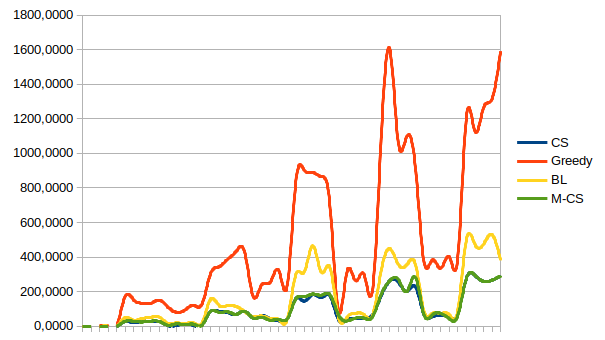
\includegraphics[width=0.65\textwidth]{"data/disp_primeros.png"}
    \caption{Dispersión por archivo de \textit{CS}, \textit{M-CS}, \textit{BL} y \textit{Greedy}}
    \label{fig:dispPrimeros}
\end{figure}

Como se aprecia, ambos algoritmos desarrollados en esta práctica son bastante similares, esto ya se demostró en las anteriores tablas, donde se expusieron los resultados.

En los valles que se aprecian en la dispersión, correspondiente a aquellos casos de menor $m$, tanto la búsqueda local como los \textit{CS}s son muy similares, en cambio, el voraz siempre mantiene la distancia, destacando por la alta dispersión obtenida en comparación con el resto.

Ahora bien, si nos fijamos en la figura \ref{fig:disp_mejores}, tenemos la dispersión de los mejores algoritmos desarrollados en la totalidad de la asignatura, siendo estos el \textit{CS} y el \textit{ILS-BL}.

\begin{figure}[H]
    \centering
    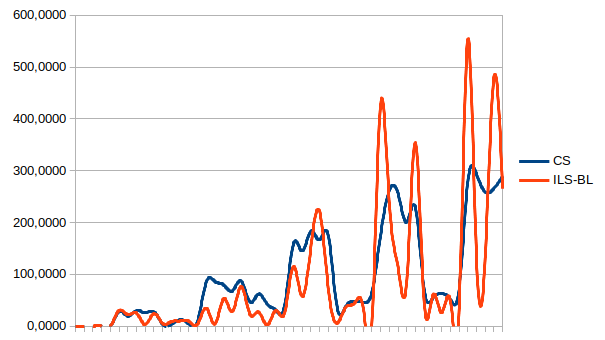
\includegraphics[width=0.65\textwidth]{"data/disp_mejores.png"}
    \caption{Dispersión por archivo de los mejores algoritmos desarrollados}
    \label{fig:disp_mejores}
\end{figure}

Se puede apreciar que el comportamiento del \textit{ILS-BL} resulta mucho más errático que el del \textit{CS}. Esto deja bastante pie a la incertidumbre a la hora de predecir qué tipo de resultados vamos a obtener, ya que entre casos aparentemente similares varía mucho la misma.

En mi opinión, la figura \ref{fig:disp_mejores} es un motivo de peso para optar por usar \textit{CS} en lugar de \textit{ILS-BL}, ya que el comportamiento va a ser menos aleatorio.

Vamos ahora a visualizar una gráfica en la figura \ref{fig:tiempoTodos} para apreciar el tiempo de ejecución por archivo de los algoritmos de esta práctica junto con los de la práctica 1.

\begin{figure}[H]
    \centering
    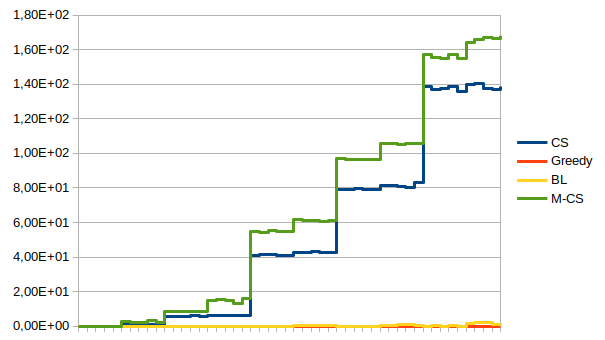
\includegraphics[width=0.65\textwidth]{"data/tiempo_primeros.png"}
    \caption{Tiempo por archivo de \textit{CS}, \textit{M-CS}, \textit{BL} y \textit{Greedy}}
    \label{fig:tiempoTodos}
\end{figure}

Podemos observar que el de mayor tiempo de ejecución resulta ser el \textit{M-CS}, como es de esperar. Sin embargo, su tiempo de ejecución es solamente un factor mayor que aquel del \textit{CS} simple, resultando ambos en el mismo orden de tiempo, es decir, el tiempo de ejecución va a escalar con el número de elementos de forma similar.

Si los comparamos con los de la primera práctica, estos tardan infinitamente más tiempo en ejecutarse.

Si vamos ahora a la figura \ref{fig:tiempoMejores}, tenemos el tiempo ejecución de los mejores algoritmos desarrollados en la totalidad de la asignatura, siendo estos el \textit{CS} y el \textit{ILS-BL}.

Hemos expresado el tiempo en escala logarítmica para que se aprecie más fácilmente.

\begin{figure}[H]
    \centering
    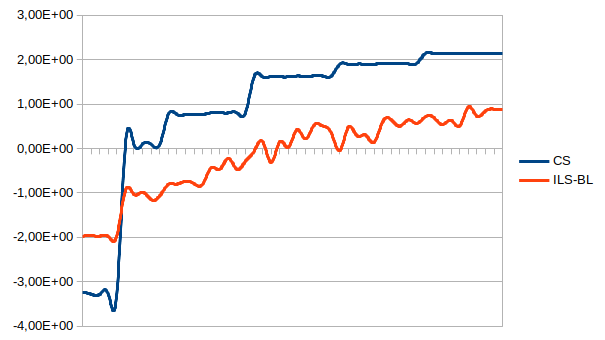
\includegraphics[width=0.65\textwidth]{"data/tiempo_mejores.png"}
    \caption{Tiempo por archivo de los mejores algoritmos desarrollados}
    \label{fig:tiempoMejores}
\end{figure}

El \textit{CS} presenta un tiempo de ejecución mayor prácticamente siempre, no obstante, ambos tienen un crecimiento similar, estando separados siempre por la misma distancia en la gráfica.

Resulta curioso las formas que realizan los tiempos por archivo, siendo mucho más predecible la del \textit{CS} frente al comportamiento errático pero creciente del \textit{ILS-BL}, un comportamiento que ya observamos con la dispersión en la figura \ref{fig:disp_mejores}, pese a que en este caso no nos lleva a usar un algoritmo frente a otro.

\newpage

\subsection{Conclusión general sobre los algoritmos estudiados}

Después de este estudio de los resultados obtenidos experimentalmente, sólo nos queda llegar a una conclusión.

Recapitulando, tenemos que de los algoritmos estudiados en esta práctica, para nuestra sorpresa, ha resultado ser mejor el \textit{CS} simple que la hibridación con el algoritmo memético.

Hemos concluido también que el \textit{ILS-BL} pese a dar mejores resultados en desviación que el \textit{CS}, presenta un comportamiento bastante aleatorio, lo que nos lleva a que si tuviéramos que usar uno de estos dos algoritmos en usa situación real usaríamos el \textit{CS}, pese a la penalización en tiempo que esto supone.

Realizando esta práctica hemos descubierto que el \textit{CS} puede ser muy preferible a nivel de desviación y tiempo que los algoritmos genéticos y los multiarranques.








\end{document}